\documentclass[11pt,a4paper,]{article}
\usepackage{lmodern}

\usepackage{amssymb,amsmath}
\usepackage{ifxetex,ifluatex}
\usepackage{fixltx2e} % provides \textsubscript
\ifnum 0\ifxetex 1\fi\ifluatex 1\fi=0 % if pdftex
  \usepackage[T1]{fontenc}
  \usepackage[utf8]{inputenc}
\else % if luatex or xelatex
  \usepackage{unicode-math}
  \defaultfontfeatures{Ligatures=TeX,Scale=MatchLowercase}
\fi
% use upquote if available, for straight quotes in verbatim environments
\IfFileExists{upquote.sty}{\usepackage{upquote}}{}
% use microtype if available
\IfFileExists{microtype.sty}{%
\usepackage[]{microtype}
\UseMicrotypeSet[protrusion]{basicmath} % disable protrusion for tt fonts
}{}
\PassOptionsToPackage{hyphens}{url} % url is loaded by hyperref
\usepackage[unicode=true]{hyperref}
\hypersetup{
            pdftitle={Report},
            pdfborder={0 0 0},
            breaklinks=true}
\urlstyle{same}  % don't use monospace font for urls
\usepackage{geometry}
\geometry{a4paper, centering, text={16cm,24cm}}
\usepackage[style=authoryear-comp,]{biblatex}
\addbibresource{references.bib}
\usepackage{color}
\usepackage{fancyvrb}
\newcommand{\VerbBar}{|}
\newcommand{\VERB}{\Verb[commandchars=\\\{\}]}
\DefineVerbatimEnvironment{Highlighting}{Verbatim}{commandchars=\\\{\}}
% Add ',fontsize=\small' for more characters per line
\usepackage{framed}
\definecolor{shadecolor}{RGB}{248,248,248}
\newenvironment{Shaded}{\begin{snugshade}}{\end{snugshade}}
\newcommand{\AlertTok}[1]{\textcolor[rgb]{0.94,0.16,0.16}{#1}}
\newcommand{\AnnotationTok}[1]{\textcolor[rgb]{0.56,0.35,0.01}{\textbf{\textit{#1}}}}
\newcommand{\AttributeTok}[1]{\textcolor[rgb]{0.77,0.63,0.00}{#1}}
\newcommand{\BaseNTok}[1]{\textcolor[rgb]{0.00,0.00,0.81}{#1}}
\newcommand{\BuiltInTok}[1]{#1}
\newcommand{\CharTok}[1]{\textcolor[rgb]{0.31,0.60,0.02}{#1}}
\newcommand{\CommentTok}[1]{\textcolor[rgb]{0.56,0.35,0.01}{\textit{#1}}}
\newcommand{\CommentVarTok}[1]{\textcolor[rgb]{0.56,0.35,0.01}{\textbf{\textit{#1}}}}
\newcommand{\ConstantTok}[1]{\textcolor[rgb]{0.00,0.00,0.00}{#1}}
\newcommand{\ControlFlowTok}[1]{\textcolor[rgb]{0.13,0.29,0.53}{\textbf{#1}}}
\newcommand{\DataTypeTok}[1]{\textcolor[rgb]{0.13,0.29,0.53}{#1}}
\newcommand{\DecValTok}[1]{\textcolor[rgb]{0.00,0.00,0.81}{#1}}
\newcommand{\DocumentationTok}[1]{\textcolor[rgb]{0.56,0.35,0.01}{\textbf{\textit{#1}}}}
\newcommand{\ErrorTok}[1]{\textcolor[rgb]{0.64,0.00,0.00}{\textbf{#1}}}
\newcommand{\ExtensionTok}[1]{#1}
\newcommand{\FloatTok}[1]{\textcolor[rgb]{0.00,0.00,0.81}{#1}}
\newcommand{\FunctionTok}[1]{\textcolor[rgb]{0.00,0.00,0.00}{#1}}
\newcommand{\ImportTok}[1]{#1}
\newcommand{\InformationTok}[1]{\textcolor[rgb]{0.56,0.35,0.01}{\textbf{\textit{#1}}}}
\newcommand{\KeywordTok}[1]{\textcolor[rgb]{0.13,0.29,0.53}{\textbf{#1}}}
\newcommand{\NormalTok}[1]{#1}
\newcommand{\OperatorTok}[1]{\textcolor[rgb]{0.81,0.36,0.00}{\textbf{#1}}}
\newcommand{\OtherTok}[1]{\textcolor[rgb]{0.56,0.35,0.01}{#1}}
\newcommand{\PreprocessorTok}[1]{\textcolor[rgb]{0.56,0.35,0.01}{\textit{#1}}}
\newcommand{\RegionMarkerTok}[1]{#1}
\newcommand{\SpecialCharTok}[1]{\textcolor[rgb]{0.00,0.00,0.00}{#1}}
\newcommand{\SpecialStringTok}[1]{\textcolor[rgb]{0.31,0.60,0.02}{#1}}
\newcommand{\StringTok}[1]{\textcolor[rgb]{0.31,0.60,0.02}{#1}}
\newcommand{\VariableTok}[1]{\textcolor[rgb]{0.00,0.00,0.00}{#1}}
\newcommand{\VerbatimStringTok}[1]{\textcolor[rgb]{0.31,0.60,0.02}{#1}}
\newcommand{\WarningTok}[1]{\textcolor[rgb]{0.56,0.35,0.01}{\textbf{\textit{#1}}}}
\usepackage{longtable,booktabs}
% Fix footnotes in tables (requires footnote package)
\IfFileExists{footnote.sty}{\usepackage{footnote}\makesavenoteenv{long table}}{}
\usepackage{graphicx,grffile}
\makeatletter
\def\maxwidth{\ifdim\Gin@nat@width>\linewidth\linewidth\else\Gin@nat@width\fi}
\def\maxheight{\ifdim\Gin@nat@height>\textheight\textheight\else\Gin@nat@height\fi}
\makeatother
% Scale images if necessary, so that they will not overflow the page
% margins by default, and it is still possible to overwrite the defaults
% using explicit options in \includegraphics[width, height, ...]{}
\setkeys{Gin}{width=\maxwidth,height=\maxheight,keepaspectratio}
\IfFileExists{parskip.sty}{%
\usepackage{parskip}
}{% else
\setlength{\parindent}{0pt}
\setlength{\parskip}{6pt plus 2pt minus 1pt}
}
\setlength{\emergencystretch}{3em}  % prevent overfull lines
\providecommand{\tightlist}{%
  \setlength{\itemsep}{0pt}\setlength{\parskip}{0pt}}
\setcounter{secnumdepth}{5}

% set default figure placement to htbp
\makeatletter
\def\fps@figure{htbp}
\makeatother


\title{Report}

%% MONASH STUFF

%% CAPTIONS
\RequirePackage{caption}
\DeclareCaptionStyle{italic}[justification=centering]
 {labelfont={bf},textfont={it},labelsep=colon}
\captionsetup[figure]{style=italic,format=hang,singlelinecheck=true}
\captionsetup[table]{style=italic,format=hang,singlelinecheck=true}


%% FONT
\RequirePackage{bera}
\RequirePackage[charter,expert,sfscaled]{mathdesign}
\RequirePackage{fontawesome}

%% HEADERS AND FOOTERS
\RequirePackage{fancyhdr}
\pagestyle{fancy}
\rfoot{\Large\sffamily\raisebox{-0.1cm}{\textbf{\thepage}}}
\makeatletter
\lhead{\textsf{\expandafter{\@title}}}
\makeatother
\rhead{}
\cfoot{}
\setlength{\headheight}{15pt}
\renewcommand{\headrulewidth}{0.4pt}
\renewcommand{\footrulewidth}{0.4pt}
\fancypagestyle{plain}{%
\fancyhf{} % clear all header and footer fields
\fancyfoot[C]{\sffamily\thepage} % except the center
\renewcommand{\headrulewidth}{0pt}
\renewcommand{\footrulewidth}{0pt}}

%% MATHS
\RequirePackage{bm,amsmath}
\allowdisplaybreaks

%% GRAPHICS
\RequirePackage{graphicx}
\setcounter{topnumber}{2}
\setcounter{bottomnumber}{2}
\setcounter{totalnumber}{4}
\renewcommand{\topfraction}{0.85}
\renewcommand{\bottomfraction}{0.85}
\renewcommand{\textfraction}{0.15}
\renewcommand{\floatpagefraction}{0.8}


%\RequirePackage[section]{placeins}

%% SECTION TITLES


%% SECTION TITLES (NEW: Changing sections and subsections color)
\RequirePackage[compact,sf,bf]{titlesec}
\titleformat*{\section}{\Large\sf\bfseries\color[rgb]{0.8, 0.7, 0.1 }}
\titleformat*{\subsection}{\large\sf\bfseries\color[rgb]{0.8, 0.7, 0.1 }}
\titleformat*{\subsubsection}{\sf\bfseries\color[rgb]{0.8, 0.7, 0.1 }}
\titlespacing{\section}{0pt}{2ex}{.5ex}
\titlespacing{\subsection}{0pt}{1.5ex}{0ex}
\titlespacing{\subsubsection}{0pt}{.5ex}{0ex}


%% TITLE PAGE
\def\Date{\number\day}
\def\Month{\ifcase\month\or
 January\or February\or March\or April\or May\or June\or
 July\or August\or September\or October\or November\or December\fi}
\def\Year{\number\year}

%% LINE AND PAGE BREAKING
\sloppy
\clubpenalty = 10000
\widowpenalty = 10000
\brokenpenalty = 10000
\RequirePackage{microtype}

%% PARAGRAPH BREAKS
\setlength{\parskip}{1.4ex}
\setlength{\parindent}{0em}

%% HYPERLINKS
\RequirePackage{xcolor} % Needed for links
\definecolor{darkblue}{rgb}{0,0,.6}
\RequirePackage{url}

\makeatletter
\@ifpackageloaded{hyperref}{}{\RequirePackage{hyperref}}
\makeatother
\hypersetup{
     citecolor=0 0 0,
     breaklinks=true,
     bookmarksopen=true,
     bookmarksnumbered=true,
     linkcolor=darkblue,
     urlcolor=blue,
     citecolor=darkblue,
     colorlinks=true}

\usepackage[showonlyrefs]{mathtools}
\usepackage[no-weekday]{eukdate}

%% BIBLIOGRAPHY

\makeatletter
\@ifpackageloaded{biblatex}{}{\usepackage[style=authoryear-comp, backend=biber, natbib=true]{biblatex}}
\makeatother
\ExecuteBibliographyOptions{bibencoding=utf8,minnames=1,maxnames=3, maxbibnames=99,dashed=false,terseinits=true,giveninits=true,uniquename=false,uniquelist=false,doi=false, isbn=false,url=true,sortcites=false}

\DeclareFieldFormat{url}{\texttt{\url{#1}}}
\DeclareFieldFormat[article]{pages}{#1}
\DeclareFieldFormat[inproceedings]{pages}{\lowercase{pp.}#1}
\DeclareFieldFormat[incollection]{pages}{\lowercase{pp.}#1}
\DeclareFieldFormat[article]{volume}{\mkbibbold{#1}}
\DeclareFieldFormat[article]{number}{\mkbibparens{#1}}
\DeclareFieldFormat[article]{title}{\MakeCapital{#1}}
\DeclareFieldFormat[article]{url}{}
%\DeclareFieldFormat[book]{url}{}
%\DeclareFieldFormat[inbook]{url}{}
%\DeclareFieldFormat[incollection]{url}{}
%\DeclareFieldFormat[inproceedings]{url}{}
\DeclareFieldFormat[inproceedings]{title}{#1}
\DeclareFieldFormat{shorthandwidth}{#1}
%\DeclareFieldFormat{extrayear}{}
% No dot before number of articles
\usepackage{xpatch}
\xpatchbibmacro{volume+number+eid}{\setunit*{\adddot}}{}{}{}
% Remove In: for an article.
\renewbibmacro{in:}{%
  \ifentrytype{article}{}{%
  \printtext{\bibstring{in}\intitlepunct}}}

\AtEveryBibitem{\clearfield{month}}
\AtEveryCitekey{\clearfield{month}}

\makeatletter
\DeclareDelimFormat[cbx@textcite]{nameyeardelim}{\addspace}
\makeatother

\author{\sf\Large\textbf{ Yiru Wang}\\ {\sf\large section1\\[0.5cm]} \sf\Large\textbf{ Kexin Xu}\\ {\sf\large section2\\[0.5cm]} \sf\Large\textbf{ Ruiqi Tang}\\ {\sf\large section3\\[0.5cm]}}

\date{\sf\Date~\Month~\Year}
\makeatletter
\lfoot{\sf Wang, Xu, Tang: \@date}
\makeatother


%%%% PAGE STYLE FOR FRONT PAGE OF REPORTS

\makeatletter
\def\organization#1{\gdef\@organization{#1}}
\def\telephone#1{\gdef\@telephone{#1}}
\def\email#1{\gdef\@email{#1}}
\makeatother
  \organization{Australian Government COVID19}

  \def\name{Our consultancy \newline Yiru Wang \&\newline Kexin XU \&\newline Ruiqi Tang}

  \telephone{(03) 9905 2478}

  \email{questions@company.com}                 %NEW: New email addresss

\def\webaddress{\url{http://company.com/stats/consulting/}} %NEW: URl
\def\abn{12 377 614 630}                                    % NEW: ABN
\def\logo{\includegraphics[width=6cm]{Figures/logo}}  %NEW: Changing logo
\def\extraspace{\vspace*{1.6cm}}
\makeatletter
\def\contactdetails{\faicon{phone} & \@telephone \\
                    \faicon{envelope} & \@email}
\makeatother

%%%% FRONT PAGE OF REPORTS

\def\reporttype{Report for}

\long\def\front#1#2#3{
\newpage
\begin{singlespacing}
\thispagestyle{empty}
\vspace*{-1.4cm}
\hspace*{-1.4cm}
\hbox to 16cm{
  \hbox to 6.5cm{\vbox to 14cm{\vbox to 25cm{
    \logo
    \vfill
    \parbox{6.3cm}{\raggedright
      \sf\color[rgb]{0.8, 0.7, 0.1 }    % NEW color 
      {\large\textbf{\name}}\par
      \vspace{.7cm}
      \tabcolsep=0.12cm\sf\small
      \begin{tabular}{@{}ll@{}}\contactdetails
      \end{tabular}
      \vspace*{0.3cm}\par
      ABN: \abn\par
    }
  }\vss}\hss}
  \hspace*{0.2cm}
  \hbox to 1cm{\vbox to 14cm{\rule{4pt}{26.8cm}\vss}\hss\hfill}  %NEW: Thicker line
  \hbox to 10cm{\vbox to 14cm{\vbox to 25cm{   
      \vspace*{3cm}\sf\raggedright
      \parbox{11cm}{\sf\raggedright\baselineskip=1.2cm
         \fontsize{24.88}{30}\color[rgb]{0, 0.29, 0.55}\sf\textbf{#1}}   % NEW: title color blue
      \par
      \vfill
      \large
      \vbox{\parskip=0.8cm #2}\par
      \vspace*{2cm}\par
      \reporttype\\[0.3cm]
      \hbox{#3}%\\[2cm]\
      \vspace*{1cm}
      {\large\sf\textbf{\Date~\Month~\Year}}
   }\vss}
  }}
\end{singlespacing}
\newpage
}

\makeatletter
\def\titlepage{\front{\expandafter{\@title}}{\@author}{\@organization}}
\makeatother

\usepackage{setspace}
\setstretch{1.5}

%% Any special functions or other packages can be loaded here.
\usepackage{float} \floatplacement{figure}{H} \floatplacement{table}{H}
<<<<<<< HEAD
\usepackage{booktabs}
\usepackage{longtable}
\usepackage{array}
\usepackage{multirow}
\usepackage{wrapfig}
\usepackage{float}
\usepackage{colortbl}
\usepackage{pdflscape}
\usepackage{tabu}
\usepackage{threeparttable}
\usepackage{threeparttablex}
\usepackage[normalem]{ulem}
\usepackage{makecell}
\usepackage{xcolor}
=======
>>>>>>> ruiqi_tang


\begin{document}
\titlepage

<<<<<<< HEAD
=======
library(plotly)
library(kableExtra)
```

\clearpage

\section*{State}

In this section, the number of victims of various crimes in eight Australian states and the number (and rate) of victims per 100,000 people will be analyzed from 2010 to 2019, and the types of crimes with the most victims will be analyzed.

\begin{figure}
\centering
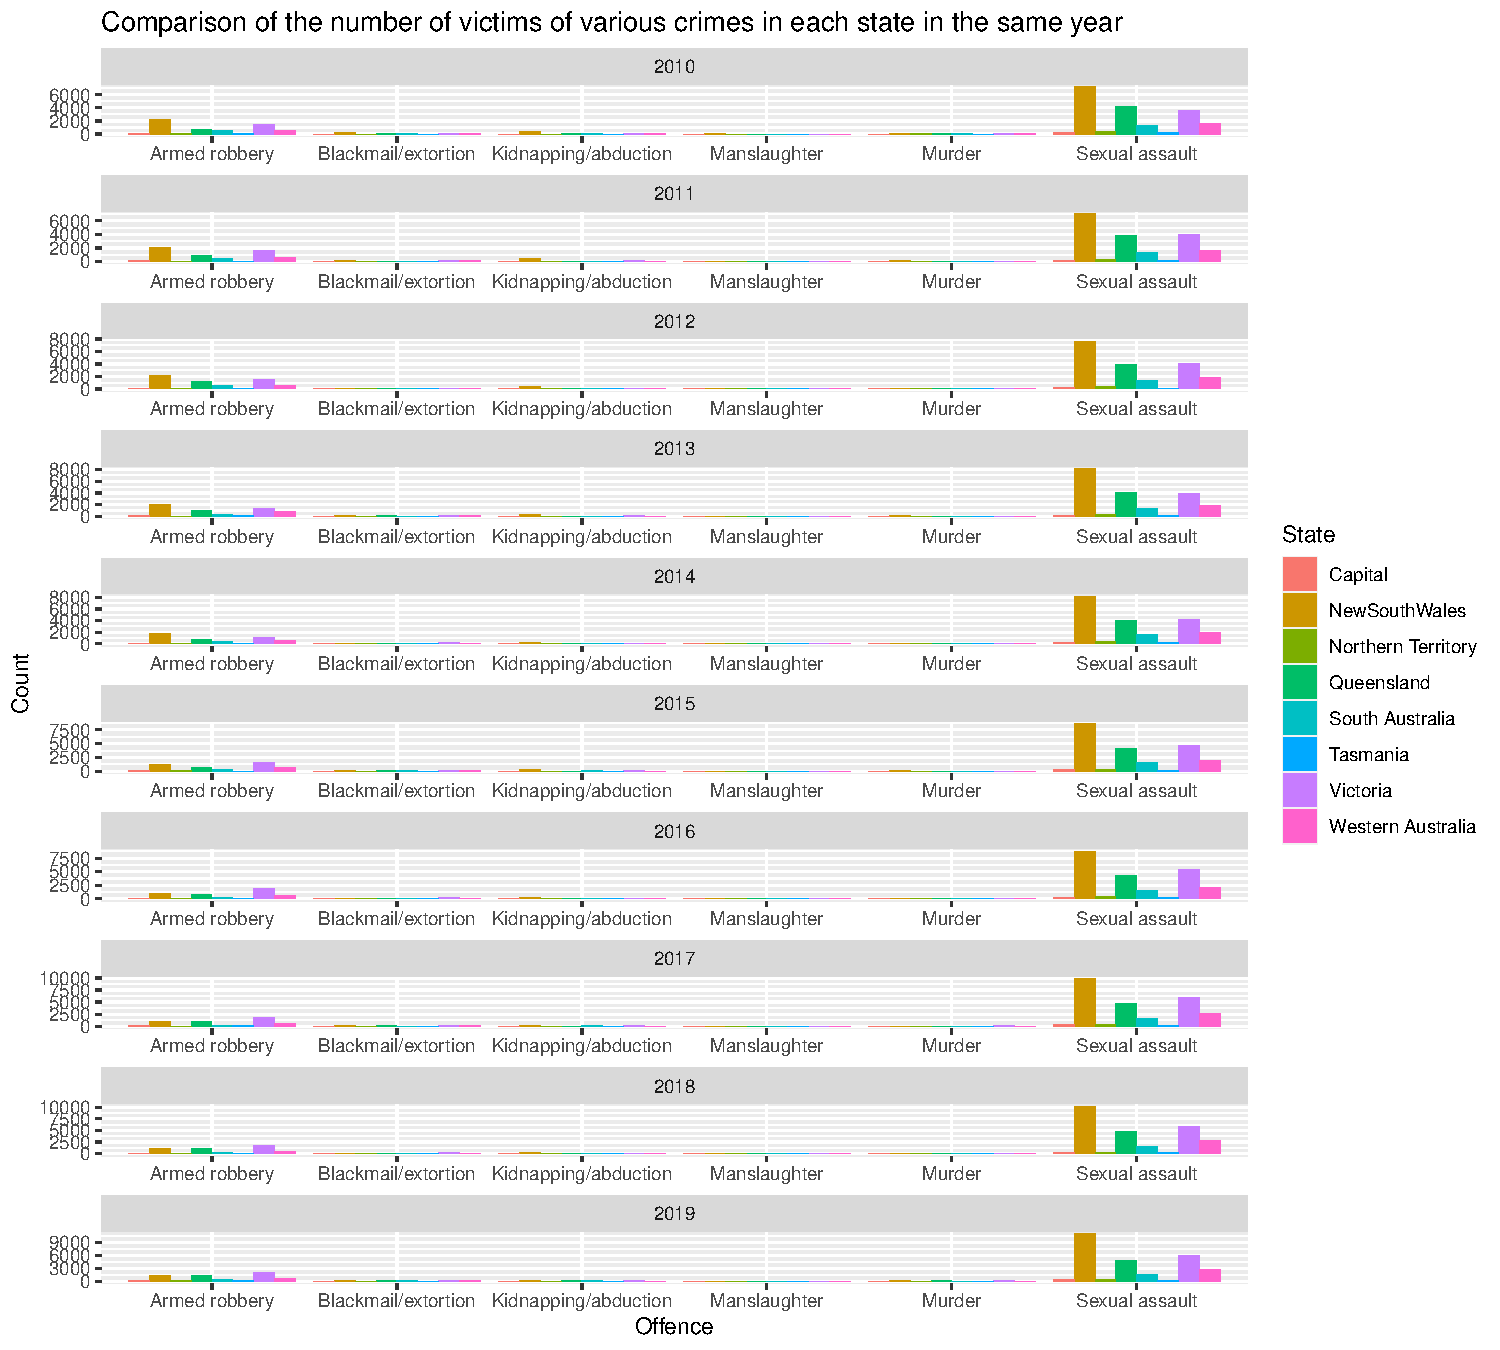
\includegraphics{report_files/figure-latex/plot1-1.pdf}
\caption{\label{fig:plot1}Comparison of the number of victims of various crimes in each state in the same year}
\end{figure}

As can be clearly seen in Figure \ref{fig:plot1}, the number of victims of sexual assault and armed robbery was the largest in the same year.

\begin{figure}
\centering
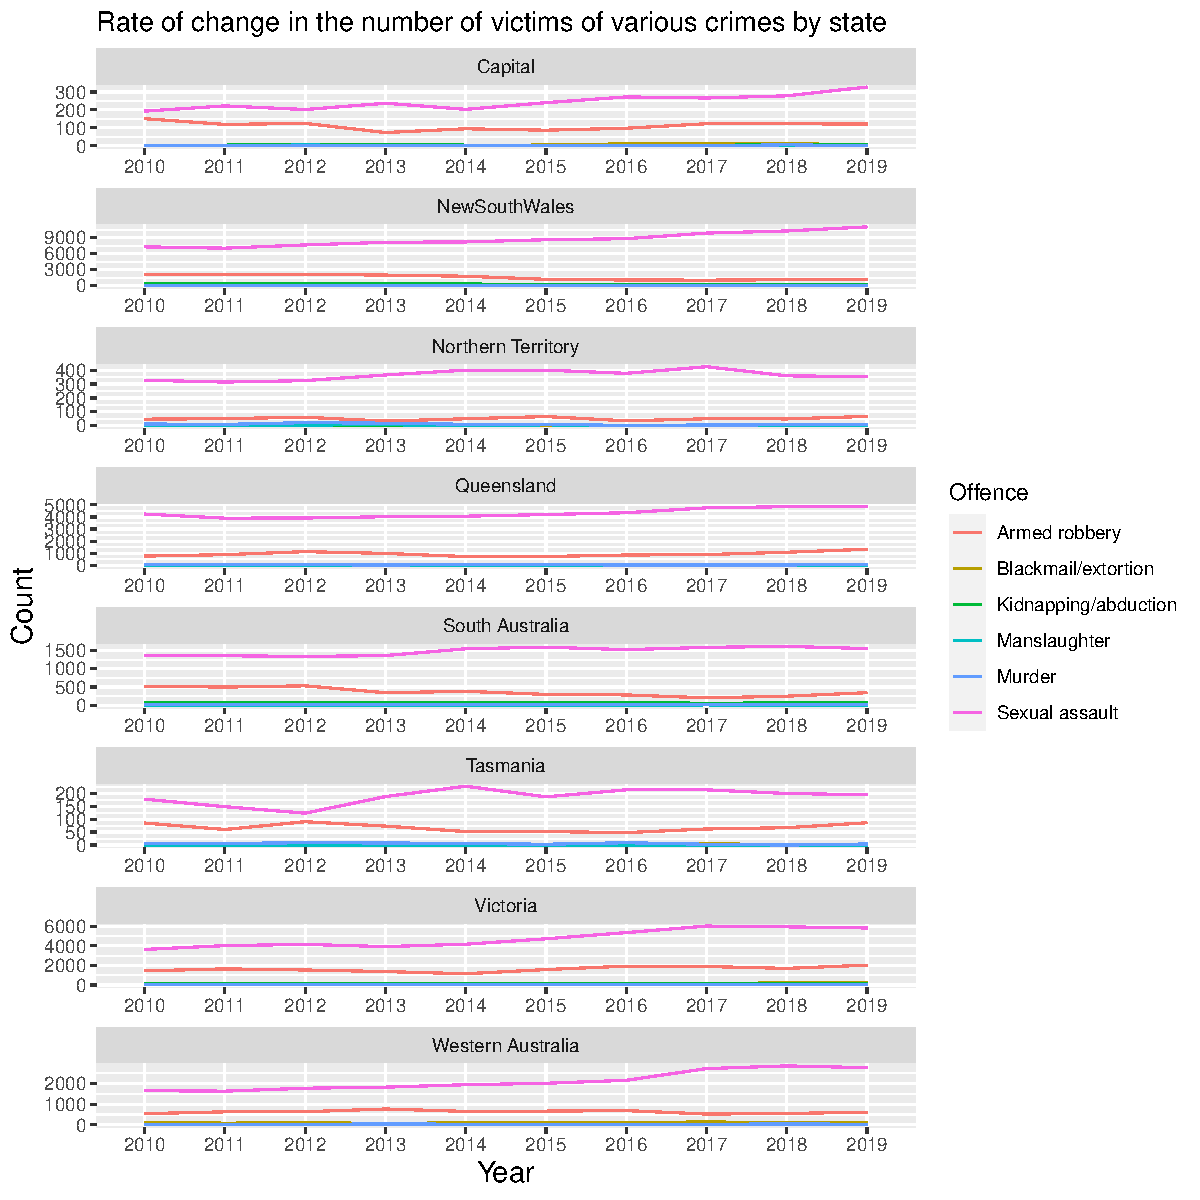
\includegraphics{report_files/figure-latex/plot2-1.pdf}
\caption{\label{fig:plot2}Rate of change in the number of victims of various crimes by state}
\end{figure}

Figure \ref{fig:plot2} shows the change in the number of crime victims by state over 10 years.Sexual assault and armed robbery are the most victimized crime categories in every state, while other crimes are victimized in relatively small numbers.

\begin{table}

\caption{\label{tab:table1}Ten-year rate of change in the number of victims of various crimes by state}
\centering
\begin{tabular}[t]{lrrrrrr}
\toprule
State & robbery\_rate & robbery\_change & Sexual assault\_rate & Sexual assault\_change & Murder\_rate & Murder\_change\\
\midrule
Capital & -19.867550 & -30 & 69.430052 & 134 & -100.000000 & -3\\
NewSouthWales & -43.953488 & -945 & 51.451369 & 3740 & 4.109589 & 3\\
Northern Territory & 43.478261 & 20 & 7.926829 & 26 & -9.090909 & -1\\
Queensland & 73.246753 & 564 & 14.626091 & 620 & -2.083333 & -1\\
South Australia & -34.482759 & -180 & 13.719736 & 187 & -33.333333 & -5\\
\addlinespace
Tasmania & 1.176471 & 1 & 9.604520 & 17 & -33.333333 & -2\\
Victoria & 40.751043 & 586 & 60.622761 & 2200 & 19.148936 & 9\\
Western Australia & 13.358071 & 72 & 67.412334 & 1115 & -10.000000 & -3\\
\bottomrule
\end{tabular}
\end{table}

\begin{table}

\caption{\label{tab:table2}Ten-year rate of change in the number of victims of various crimes by state}
\centering
\begin{tabular}[t]{lrrrrrr}
\toprule
State & extortion\_rate & extortion\_change & Manslaughter\_rate & Manslaughter\_change & Kidnapping\_rate & Kidnapping\_change\\
\midrule
Capital & Inf & 6 & NaN & 0 & Inf & 7\\
NewSouthWales & -46.24277 & -80 & 18.18182 & 2 & -31.610942 & -104\\
Northern Territory & Inf & 3 & -100.00000 & -3 & NaN & 0\\
Queensland & 108.69565 & 50 & -57.14286 & -4 & -13.235294 & -9\\
South Australia & 96.77419 & 30 & NaN & 0 & -9.230769 & -6\\
\addlinespace
Tasmania & NaN & 0 & NaN & 0 & Inf & 3\\
Victoria & 43.06569 & 59 & 366.66667 & 11 & 36.206897 & 42\\
Western Australia & 20.00000 & 18 & 0.00000 & 0 & 21.052632 & 4\\
\bottomrule
\end{tabular}
\end{table}

Table \ref{tab:table1} and Table \ref{tab:table2} show the ten-year change and rate of change in the number of victims of the above six types of crime. Sexual assault was the only crime category in which victims increased in all states, with increases of 51.45 per cent in New South Wales, 67.4 per cent in Western Australia, 60.6 per cent in Victoria and 69.4 per cent in the Australian Capital Territory. Victoria was also the only state to see an increase in the number of victims of all six types of crime.

\begin{figure}
\centering
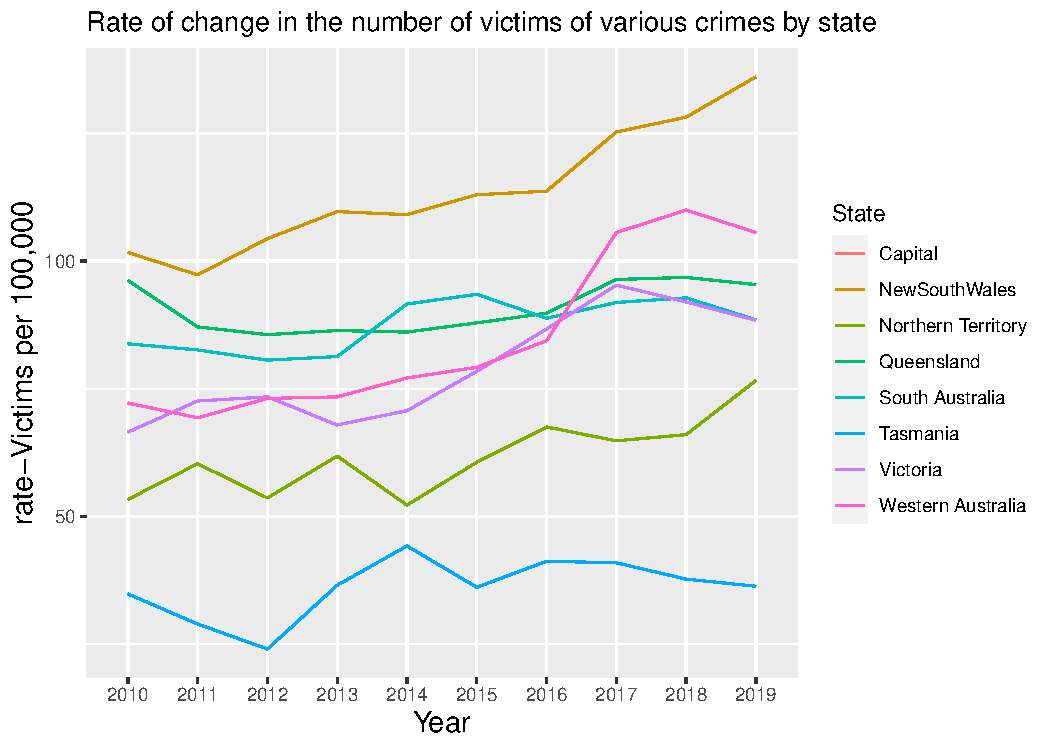
\includegraphics{report_files/figure-latex/plot3-1.pdf}
\caption{\label{fig:plot3}The rate of change in the rate of various crime victims by state}
\end{figure}

Since sexual assault is the most victimized crime category and the only one with a 10-year increase in the number of victims in all eight states, we will look at it separately.

Figure \ref{fig:plot3} shows how the rate of victims of sexual assault (the number of victims per 100,000 people) changed in eight states from 2010 to 2019. New South Wales had the highest rate of victims, while Tasmania had the lowest. Rates of sexual assault victims fluctuated in most states.

\begin{table}

\caption{\label{tab:table3}A 10-year change in the proportion of victims of sexual assault}
\centering
\begin{tabular}[t]{lrr}
\toprule
State & 2010-2011 & rate\_change\\
\midrule
NewSouthWales & 34.4 & 33.8249754\\
Victoria & 21.9 & 32.9323308\\
Queensland & -0.8 & -0.8316008\\
South Australia & 4.7 & 5.6085919\\
Western Australia & 33.4 & 46.2603878\\
\addlinespace
Tasmania & 1.5 & 4.3103448\\
Northern Territory & 23.3 & 43.7148218\\
Capital & 23.3 & 43.7148218\\
\bottomrule
\end{tabular}
\end{table}

Table \ref{tab:table3} shows the change of the proportion of victims of sexual assault in all states. Except Queensland, the proportion of victims in all states is increasing. The increase of the proportion of victims in Western Australia, Northern Territory, Australian Capital Territory is more than 40\%. Western Australia saw the highest increase of 46.3\%.

Based on the above analysis, we can conclude that the state with the most victims among the eight states is New South Wales, and the type of crime with the most victims is sexual assault. The number of victims of sexual assault in each state has increased over the past 10 years, and Western Australia has even increased by 46.3\%. Only Queensland has a decrease in the number of victims of sexual assault, which shows that Queensland attaches importance to such crimes.

\clearpage

\section*{Gender}

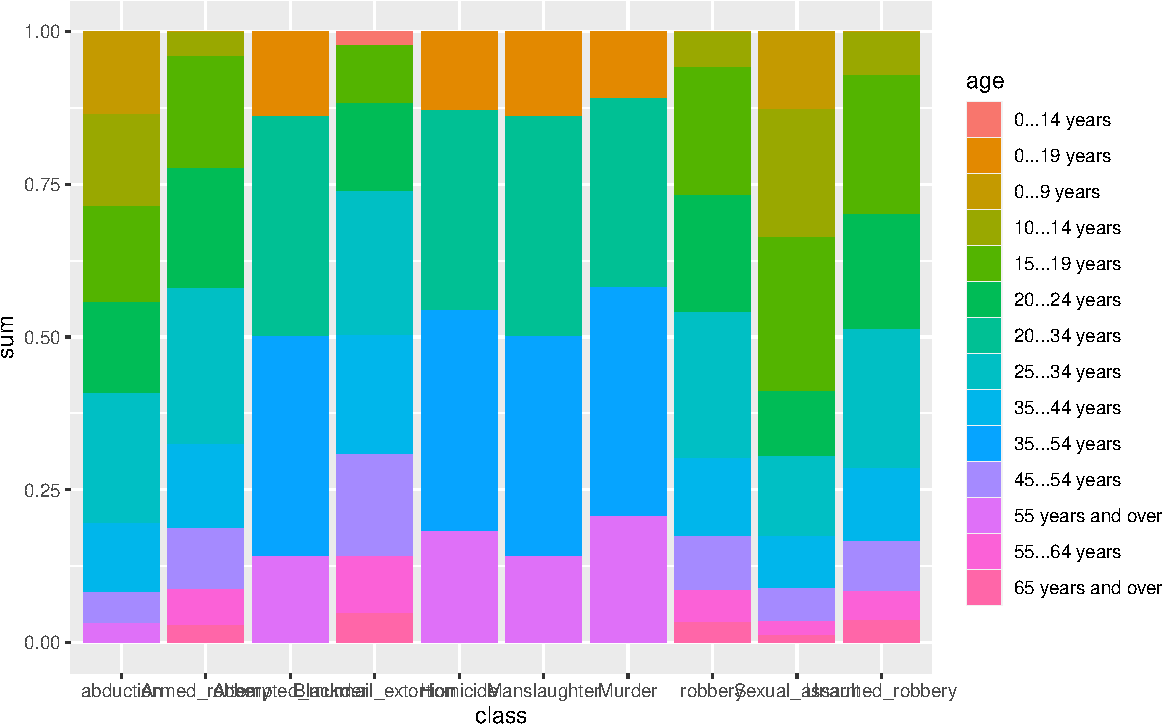
\includegraphics{report_files/figure-latex/unnamed-chunk-5-1.pdf}

\begin{itemize}
\tightlist
\item
  On the whole, it shows an upward trend year by year recently.\\
\item
  The number of female victims is much higher than that of male victims, almost twice.
\end{itemize}

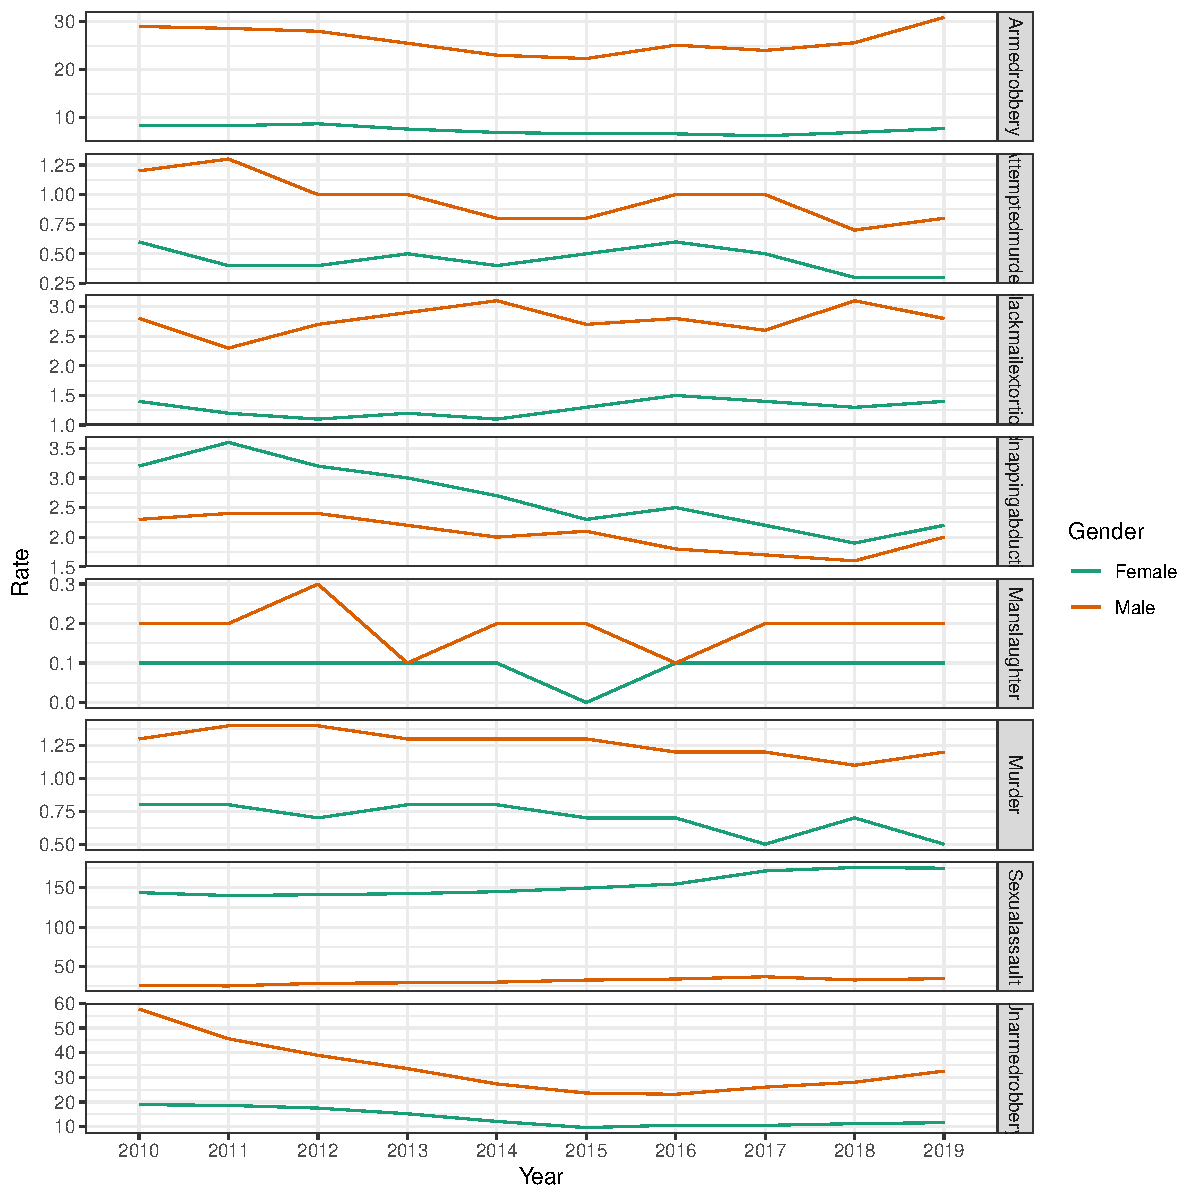
\includegraphics{report_files/figure-latex/unnamed-chunk-6-1.pdf}

\begin{itemize}
\tightlist
\item
  With the exception of sexual assault and kidnapping, the majority of victims are men.
\item
  The vast majority of cases are sexual assaults.\\
\item
  The number of robberies among the remaining crime categories is also considerable. (Including both armed and unarmed)\\
\item
  Possible reasons:

  \begin{itemize}
  \tightlist
  \item
    Women generally have stronger safety awareness
  \item
    Women are less likely to be seen alone at night in areas where they are likely to be robbed
  \end{itemize}
\end{itemize}

According to statistics of gender-specific crimes in various countries, male victims are the majority in almost all crimes except for sex-related crimes in which more women are victims.

\begin{table}

\caption{\label{tab:unnamed-chunk-7}Sexual Assault Rate}
\centering
\begin{tabular}[t]{l|l|r}
\hline
Gender & Year & sa\_rate\\
\hline
Female & 2010 & 81.14353\\
\hline
Female & 2011 & 80.92590\\
\hline
Female & 2012 & 81.71220\\
\hline
Female & 2013 & 83.46100\\
\hline
Female & 2014 & 85.77439\\
\hline
Female & 2015 & 87.63073\\
\hline
Female & 2016 & 87.29571\\
\hline
Female & 2017 & 88.86702\\
\hline
Female & 2018 & 88.74093\\
\hline
Female & 2019 & 87.99638\\
\hline
Male & 2010 & 21.67991\\
\hline
Male & 2011 & 23.79634\\
\hline
Male & 2012 & 27.87459\\
\hline
Male & 2013 & 30.70995\\
\hline
Male & 2014 & 34.46328\\
\hline
Male & 2015 & 38.35306\\
\hline
Male & 2016 & 38.22735\\
\hline
Male & 2017 & 39.55563\\
\hline
Male & 2018 & 35.52154\\
\hline
Male & 2019 & 33.06397\\
\hline
\end{tabular}
\end{table}

Take sexual assault, female victims of sexual assault make up a very high proportion of total female victims.

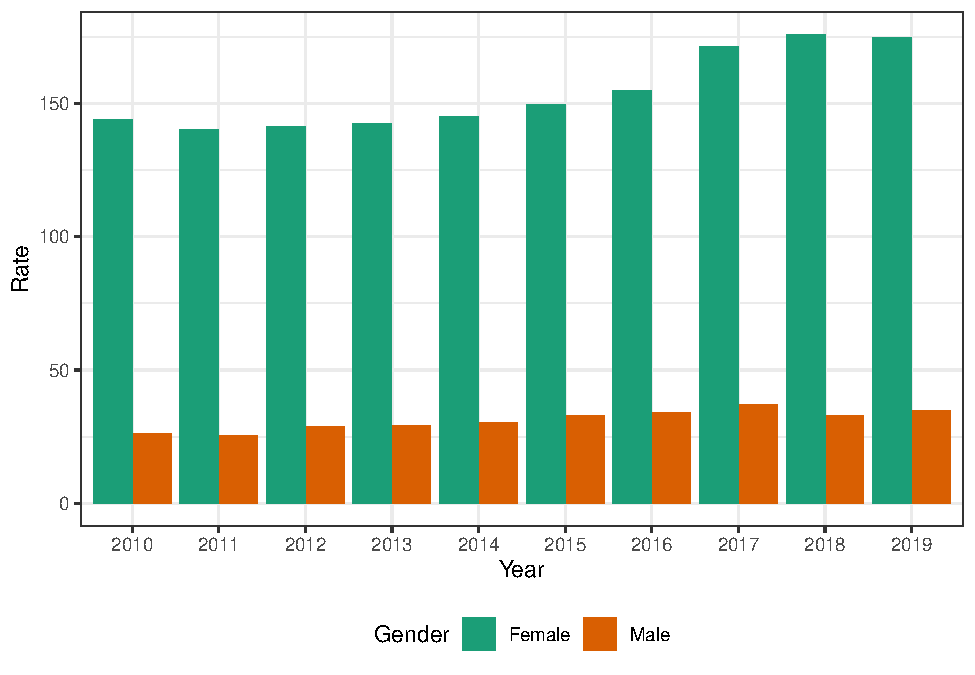
\includegraphics{report_files/figure-latex/unnamed-chunk-9-1.pdf}

\begin{itemize}
\tightlist
\item
  Rate is calculated by victim number divided by 100,000 persons.
\item
  Show an upward pattern over years.
\item
  Higher than 0.15\% in recent years which means 3 out of every 2,000 people have been sexually assaulted.
\item
  Possible reasons:

  \begin{itemize}
  \tightlist
  \item
    Women are physically vulnerable
  \item
    Men are more sexually impulsive
  \item
    Many women may choose not to report the crime

    \begin{itemize}
    \tightlist
    \item
      relationship to the offender
    \item
      confidence in the justice system
    \item
      fear of revenge
    \item
      public opinion
    \end{itemize}
  \end{itemize}
\end{itemize}

ABS personal safety survey also measures the number of women who contacted the police about the most recent incident within the last 10 years. Only 13.4\% of women did so.

\clearpage

\section*{Age}
=======
\section*{State}

\section*{Gender}

\section*{Age}

\begin{center}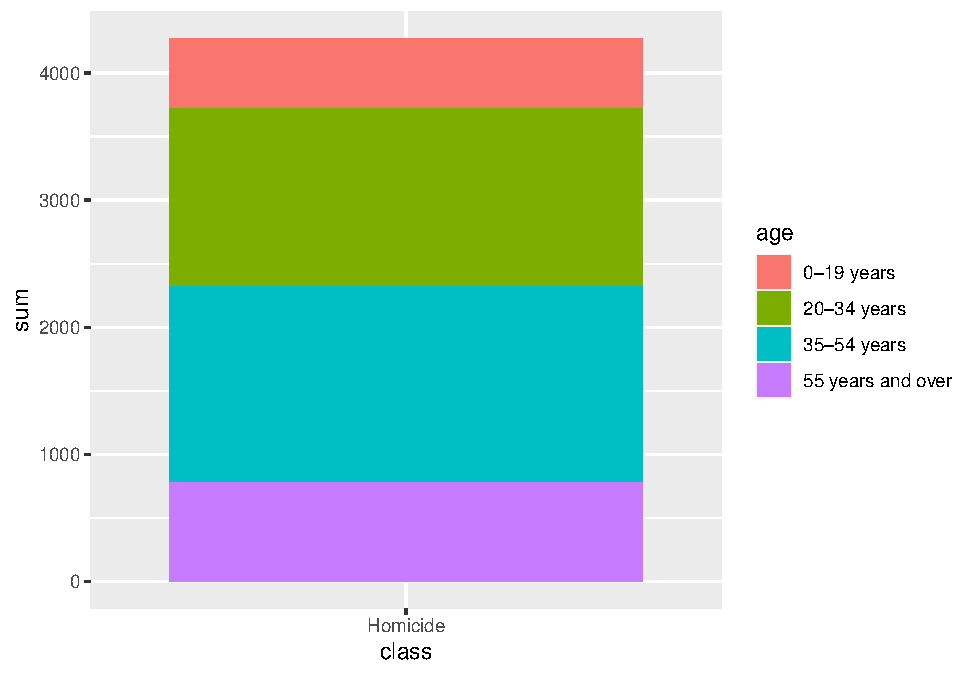
\includegraphics[width=0.5\linewidth]{report_files/figure-latex/Homicide-1} \end{center}

\begin{Shaded}
\begin{Highlighting}[]
\NormalTok{Armed\_robbery }\SpecialCharTok{\%\textgreater{}\%}
  \FunctionTok{pivot\_longer}\NormalTok{(}\AttributeTok{cols =} \StringTok{\textquotesingle{}2010\textquotesingle{}}\SpecialCharTok{:}\StringTok{\textquotesingle{}2019\textquotesingle{}}\NormalTok{,  }
                \AttributeTok{names\_to =} \StringTok{"Year"}\NormalTok{,            }
                \AttributeTok{values\_to =} \StringTok{"Count"}\NormalTok{) }\OtherTok{{-}\textgreater{}}\NormalTok{ AR\_longer}

\NormalTok{AR\_longer }\SpecialCharTok{\%\textgreater{}\%}
  \FunctionTok{pivot\_wider}\NormalTok{(}\AttributeTok{id\_cols =} \FunctionTok{c}\NormalTok{(age, Year, Count), }\AttributeTok{names\_from =}\NormalTok{ age, }\AttributeTok{values\_from =}\NormalTok{ Count) }\SpecialCharTok{\%\textgreater{}\%}
  \FunctionTok{mutate}\NormalTok{(}\AttributeTok{Year =} \FunctionTok{as\_factor}\NormalTok{(Year)) }\SpecialCharTok{\%\textgreater{}\%}
  \FunctionTok{mutate}\NormalTok{(}\AttributeTok{class =} \StringTok{"Armed\_robbery"}\NormalTok{) }\OtherTok{{-}\textgreater{}}\NormalTok{ AR\_wider}


\NormalTok{AR\_longer }\SpecialCharTok{\%\textgreater{}\%}
  \FunctionTok{group\_by}\NormalTok{(age) }\SpecialCharTok{\%\textgreater{}\%}
  \FunctionTok{summarise}\NormalTok{(}\AttributeTok{sum =} \FunctionTok{sum}\NormalTok{(Count)) }\SpecialCharTok{\%\textgreater{}\%}
  \FunctionTok{mutate}\NormalTok{(}\AttributeTok{class =} \StringTok{"Armed\_robbery"}\NormalTok{) }\SpecialCharTok{\%\textgreater{}\%}
  \FunctionTok{filter}\NormalTok{(age }\SpecialCharTok{!=} \StringTok{"Total"}\NormalTok{) }\OtherTok{{-}\textgreater{}}\NormalTok{ AR\_age}
\end{Highlighting}
\end{Shaded}

\begin{center}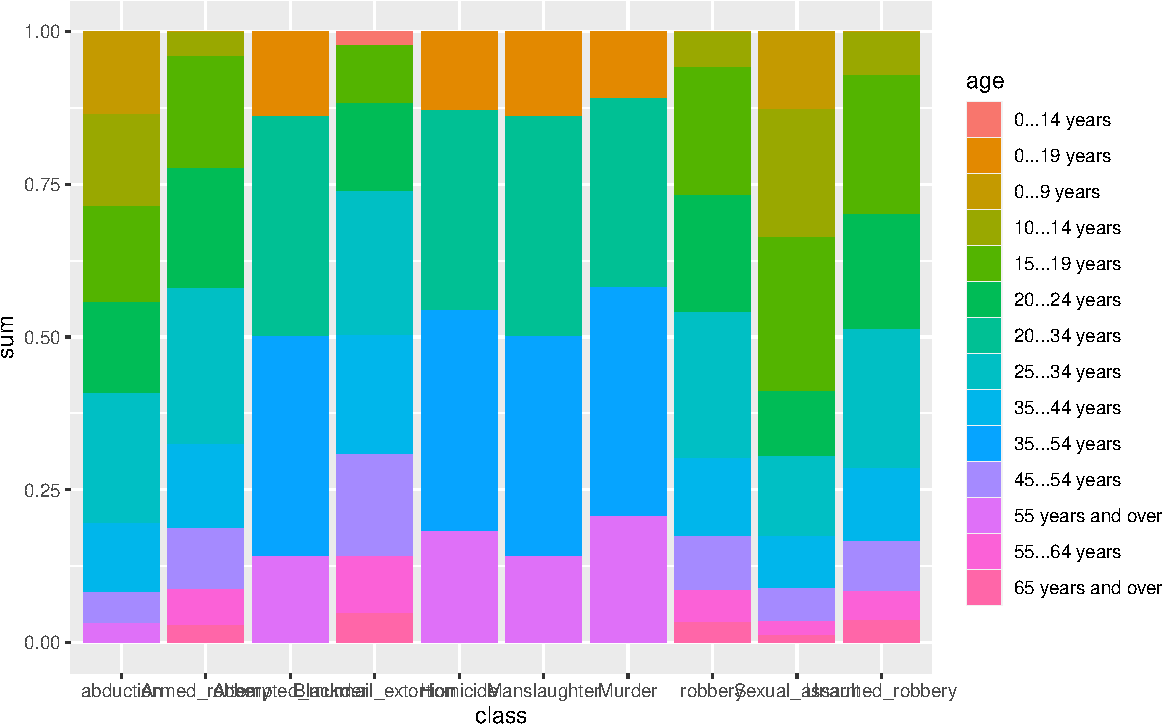
\includegraphics[width=0.5\linewidth]{report_files/figure-latex/graph-1} \end{center}

\begin{center}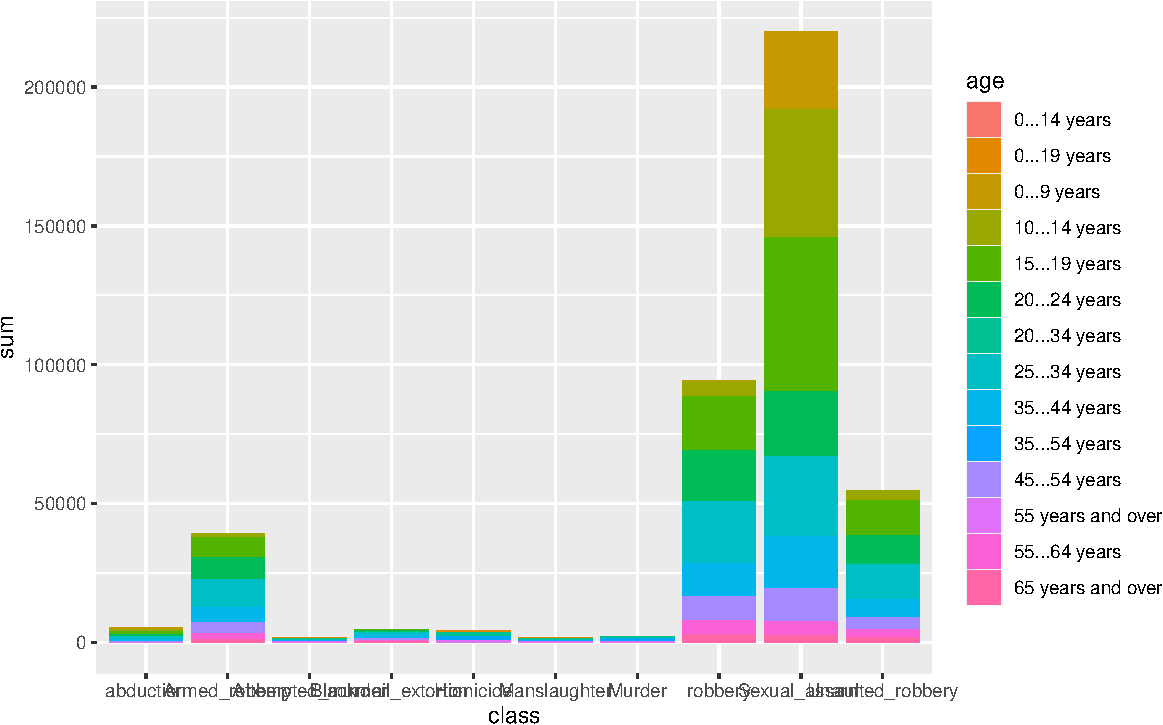
\includegraphics[width=0.5\linewidth]{report_files/figure-latex/graph-2} \end{center}

from graph, we can see that Sexual assauslt is the largest part, compared with other class
From the graph, we can see that the people who are 35-54 have bigger probability to has crimal recod
>>>>>>> ruiqi_tang

\printbibliography

\end{document}
